\documentclass[10pt,t]{beamer}
\usepackage{pslatex}
\usepackage{fontspec}
\newfontfamily\DejaSans{DejaVu Sans}
\usepackage{caption}
\usepackage{subcaption}
\usepackage{ amssymb }
\graphicspath{{graphics/}}

\usetheme[nat,dogma,totalframes=show]{Frederiksberg}

\usepackage{listings}
\usepackage{xcolor}

\definecolor{codegreen}{rgb}{0,0.6,0}
\definecolor{codegray}{rgb}{0.5,0.5,0.5}
\definecolor{codepurple}{rgb}{0.58,0,0.82}
\definecolor{backcolour}{rgb}{0.95,0.95,0.92}

\lstdefinestyle{mystyle}{
    backgroundcolor=\color{backcolour},
    commentstyle=\color{codegreen},
    keywordstyle=\color{magenta},
    numberstyle=\tiny\color{codegray},
    stringstyle=\color{codepurple},
    basicstyle=\ttfamily\footnotesize,
    breakatwhitespace=false,
    breaklines=true,
    captionpos=b,
    keepspaces=true,
    numbers=left,
    numbersep=5pt,
    showspaces=false,
    showstringspaces=false,
    showtabs=false,
    tabsize=2
}

\lstset{style=mystyle}

\usepackage{coloremoji}

\title{IFC: \normalfont{An application for dynamic evaluation and static verification of programs}}
\subtitle{}
\author{Jacob Herbst (mwr148) \&
  Matilde Broløs (jtw868)\\}
\institute[DIKU]{Institute of Computer Science (DIKU)}
\date[]{\today}

\begin{document}
\frame[plain]{\titlepage}

\begin{frame}[c]
  \begin{center}
  \frametitle{Agenda}
  \begin{itemize}
    \item Introduction
    \item Quantification in Interpreter
    \item Example programs
          \begin{itemize}
            \item[-] Div2
            \item[-] L
          \end{itemize}
    \item Division and Modulo by 0
    \item Conclusion
    \item Questions
  \end{itemize}
\end{center}
\end{frame}


\begin{frame}[c]
  \frametitle{Introduction}
  \begin{itemize}
  \item Static proving vs dynamic evaluation
    \item Hoare Triples
          $$ \{P\}s\{Q\}$$
    \item Verification Condition generation
          $$ \{WP(s,Q)\}s\{Q\}$$
  \end{itemize}
\end{frame}

\begin{frame}[c]
  \frametitle{Overview of Application🌮}
  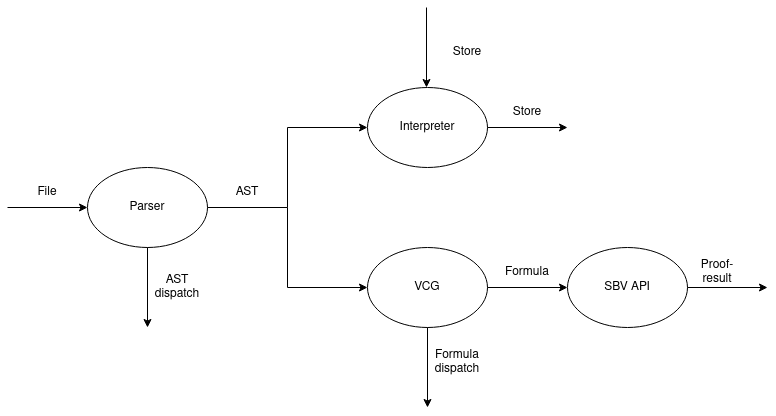
\includegraphics[width=10cm]{IFCapp}
\end{frame}


\subsection{Interpreter}\label{sec:evaluator}
The interpreter follows directly from the semantics presented in \cref{sec:Language}.
That is the intial store provided to the evalutor will be modified over the course of the program according to the semantics.
We define the \verb\Eval\ type as follows such:

\begin{lstlisting}
type STEnv = M.Map VName Integer
type Eval a = RWST () () STEnv (Either String) a
\end{lstlisting}

At the moment there is no use for neither \verb\reader\ nor \verb\writer\, however when the language in the future is extended to have procedures the reader monad will be a natural choice for the scoping rules of said procedures.
Likewise it is highly likely that the language would need to support some sort of output in the future.
The store described in \cref{sec:Language} is kept in the State \verb\STEnv\.
The store is simply a map from \texttt{VNames} to \texttt{Integers}. We want the store to be a State as the store after one monadic action should be chained with the next monadic action. This ensures that all variables are in scope for the rest of the program and hereby entails mutability.
Duly note that ghost variables will also reside in this environment but will not be mutable or even callable, as previously explained.
We make use of the error monad to resolve any runtime-errors that would arise, that is if a violation occurs, a ghost is assigned, a variable is used before it is defined, or if undefined behaviour arises such as division by 0. Semantically, the first error that occurs will be the return value of the computation.
\\~\\
Each type defined in the AST, \verb\Stmt\, \verb\FOL\, \verb\AExpr\, \verb\BExpr\ is evaluated by different functions which all operate under the \verb\Eval\ monad, which allows for a clean and modular monadic compiler. They have the following types:
%\footnote{Can we use a typeclass so they all are named eval??? Or is that too Rusty???}

\begin{lstlisting}
eval :: Stmt -> Eval ()
evalFOL :: FOL -> Eval Bool
evalBExpr :: BExpr -> Eval Bool
evalAExpr :: AExpr -> Eval Integer
\end{lstlisting}

From this we notice that all of the different constructs except for \verb\Stmt\, will produce a value, whereas \verb\Stmt\ can only produce monadic actions, in terms of modifying the store. This monadic context allows us to translate the operational semantics almost directly into Haskell code.
\cref{fig:evalS} presents the code for evaluating statements.

\begin{figure}[h]
\begin{lstlisting}
eval :: Stmt -> Eval ()
eval (Seq s1 s2) = eval s1 >> eval s2
eval (GhostAss vname a) =
    get >>= maybe (update vname a) (const _e) . M.lookup vname
eval (Assign vname a) = update vname a
eval (If c s1 s2) =
    evalBExpr c >>= \c' -> if c' then eval s1 else eval s2
eval (Asst f) = evalFOL f >>= \case
  True  -> return ()
  False -> _e
eval w@(While c invs _var s) =
  evalFOL invs >>= \case
    False -> _e
    True -> evalBExpr c >>= \case
      True -> eval s >> eval w
      False -> return ()
eval Skip = return ()
eval Fail = _e
\end{lstlisting}
\caption{Evaluator for statements.\footnote{Note that \verb\_e\ is a placeholder for the run-time errors mentioned before.}}
\label{fig:evalS}
\end{figure}

The most complex argument for equivalence between the code and the semantics is the \texttt{while} construct. \cref{fig:evalS}, line 11-16, shows how we evaluate it.
We first evaluate the invariant, to directly follow the semantical rules. Hence, when the invariant does not hold, we handle this case as abnormal termination, as per rule \textit{while-i-false} from \cref{table:semantic}, similarly to how we would do for a standard assertion.
If the invariant holds, but the loop-condition does not, we do nothing, as per rule \textit{while-false}.
Lastly if both the invariant and the loop-condition evaluates to \textit{true}, we evaluate the body, and then we evaluate the while loop again.
The other statements are simple and we treat them similarly to \texttt{while}, directly in accordance with the semantics.
\\~\\
One important note about the interpreter is that we have no good way of checking assertions which includes quantifiers. 
The reasons is that we wanted to support arbitrary precision integers.
This entails that we currently have no feasible way to check such assertions.
A potential solution would be to generate a symbolic reprensentation of the formula and try to satisfy it by using an external prover.
A downside to this approach is that the interpreter would then also require external dependencies, and not be a standalone program anymore.
All in all, this is unideal, and currently the approach is to ignore such assertions by considering them true. 
In \cref{sec:future} we describe a potential extension to \textit{While}, which could help alleviate this problem.
Non-quantified assertions are still evaluated as per the operational semantics.


\begin{frame}[containsverbatim]
  \frametitle{Program DIV2}
  $$\vdash \{x = n \land n \geq 0\} \textbf{ DIV2 } \{ 2 \times q + x = n \land 0 \leq x \land x < 2 \}$$
\begin{lstlisting}[mathescape=true]
q := $0$;
while x $>$ $1$ do
  p := $1$;
  while $2$ $\times$ p $\le$ x do
    q := q $+$ p;
    p := $2$ $\times$ p;
    x := x $-$ p;
\end{lstlisting}
Invariant of inner loop: $$2 \times q + x = n \land 0 \leq x \land 1 \leq p \land x + 2 \times (p - 1) = i \land 2 \leq i$$
\end{frame}

\begin{frame}[containsverbatim]
  \frametitle{Program DIV2}
\begin{lstlisting}[mathescape=true]
vars: [$x$]
requirements: {$x \geq 0$}
<!=_=!>
$👻n := x;$
#{$👻n \geq 0$};
$q := 0;$
while ($x > 1$) ?{$2 \times q + x = 👻n \land x \geq 0$ } !{$x$} {
   $p := 1;$
   while ($2 \times p \leq x$)
   ?{$2 \times q + x = 👻n \land 0 \leq x \land 1 \leq p \land x + 2 \times (p - 1) = i \land 2 \leq i $}
   !{$x$} {
      $q := q + p;$
      $p := 2 \times p;$
      $x := x - p;$
   };
};
#{$2 \times q + x = 👻n \land 0 \leq x \land x < 2$};
\end{lstlisting}
\end{frame}


\begin{frame}[containsverbatim]
  \frametitle{Program DIV2}
\begin{lstlisting}[mathescape=true]
vars: [$x$]
requirements: {$x \geq 0$}
<!=_=!>
$👻n := x;$
#{$👻n \geq 0$};
$q := 0;$
while ($x > 1$) ?{$2 \times q + x = 👻n \land  x \geq 0$ } !{$x$} {
   $p := 1;$
   while ($2 \times p \leq x$)
   ?{$2 \times q + x = 👻n \land 0 \leq x \land 1 \leq p \land  x + 2 \times (p - 1) = \textcolor{red}{i} \land 2 \leq \textcolor{red}{i} $}
   !{$x$} {
      $q := q + p;$
      $p := 2 \times p;$
      $x := x - p;$
   };
};
#{$2 \times q + x = 👻n \land 0 \leq x \land x < 2$};
\end{lstlisting}
\end{frame}

\begin{frame}[containsverbatim]
  \frametitle{Program DIV2}
\begin{lstlisting}[mathescape=true]
vars: [$x$]
requirements: {$x \geq 0$}
<!=_=!>
$👻n := x;$
#{$👻n \geq 0$};
$q := 0;$
while ($x > 1$) ?{$2 \times q + x = 👻n \land  x \geq 0$ } !{$x$} {
   $\textcolor{red}{i := x;}$
   $p := 1;$
   while ($2 \times p \leq x$)
   ?{$2 \times q + x = 👻n \land 0 \leq x \land 1 \leq p \land  x + 2 \times (p - 1) = \textcolor{red}{i} \land 2 \leq \textcolor{red}{i} $}
   !{$x$} {
      $q := q + p;$
      $p := 2 \times p;$
      $x := x - p;$
   };
};
#{$2 \times q + x = 👻n \land 0 \leq x \land x < 2$};
\end{lstlisting}
\end{frame}

\begin{frame}[containsverbatim]
  \frametitle{Program DIV2}
  \begin{itemize}
    \item Loop-invariant of outer loop
    \item Introduction of $i$
    \item Prove total correctness
  \end{itemize}
\end{frame}

\begin{frame}[containsverbatim]
  \frametitle{Program DIV2}
  \begin{itemize}
    \item Loop-invariant of outer loop
    \item Introduction of $i$
    \item Prove total correctness
  \end{itemize}
  \\~\\
  But what about $L$?
\end{frame}


\begin{frame}[containsverbatim]
  \frametitle{Program L}
  $$\vdash \{x \geq 0\} \textbf{ L } \{ true \}$$
\begin{lstlisting}[mathescape=true]
$ y := 0$;
while $x > 1 \lor y > 0$ do
   if $x > 0$ then
      $x := x - 1;$
      $y := y + y;$
    else
      $y := y - 1;$
\end{lstlisting}
\end{frame}

\begin{frame}[containsverbatim]
  \frametitle{Program L}
\begin{lstlisting}[mathescape=true]
vars: [$x$]
requirements: {$x \geq 0$}
<!=_=!>
$y := 1;$
while ($x > 0$ || $y > 0$) ?{$true$} !{$\textcolor{red}{\mathbf{?}}$} {
    if $x > 0$ {
        $x := x - 1;$
        $y := y + y;$
    } else {
        $y := y - 1;$
    };
};
#{$true$};
\end{lstlisting}
Problem is that first $x$ decrements while $y$ increments, then only $y$ decrements.\\
No way to express the variant.
\end{frame}

\begin{frame}[containsverbatim]
  \frametitle{Program L}
  With current methods we cannot prove termination, but dynamic evaluation terminates.
  How can we fix this?
\end{frame}

\begin{frame}[containsverbatim]
  \frametitle{Program L}
  With current methods we cannot prove termination, but dynamic evaluation terminates.
  How can we fix this?
  \\~\\
  \textcolor{red}{Introducing tuples!}
\end{frame}

\begin{frame}[containsverbatim]
  \frametitle{Program L}
\begin{lstlisting}[mathescape=true]
vars: [$x$]
requirements: {$x \geq 0$}
<!=_=!>
$y := 1;$
while ($x > 0$ || $y > 0$) ?{$true$} !{$\textcolor{red}{x , y}$} {
    if $x > 0$ {
        $x := x - 1;$
        $y := y + y;$
    } else {
        $y := y - 1;$
    };
};
#{$true$};
\end{lstlisting}
What is the meaning of this?
\end{frame}

\begin{frame}[containsverbatim]
  \frametitle{Program L}
\begin{align*}
  &\frac{
    \{I \land e \land \textcolor{blue}{v = \xi} \} s \{I \land \textcolor{blue}{v \prec \xi} \} \quad wf(\prec)
  }{
    \{I\} \texttt{ while } e \texttt{ invariant } I
          \texttt{ variant } \textcolor{blue}{v}, \prec \texttt{ do } s \{I \land \neg e\}
  }
\end{align*}
\\~\\
\\~\\
\\~\\
\\~\\
\\~\\
\\~\\
\\~\\
\\~\\
\\~\\
\\~\\
\\~\\
\\~\\
\\~\\
\\~\\
\\~\\
\\~\\
\\~\\
\\~\\
\\~\\
\end{frame}

\begin{frame}[containsverbatim]
  \frametitle{Program L}
\begin{align*}
  &\frac{
    \{I \land e \land \textcolor{blue}{v = \xi} \} s \{I \land \textcolor{blue}{v \prec \xi} \} \quad wf(\prec)
  }{
    \{I\} \texttt{ while } e \texttt{ invariant } I
          \texttt{ variant } \textcolor{blue}{v}, \prec \texttt{ do } s \{I \land \neg e\}
  }
\end{align*}
\begin{align*}
  \Downarrow &
\end{align*}
\begin{align*}
  &\frac{
    \{I \land e \land \textcolor{red}{u = \xi_{1} \land v = \xi_{2}} \} s \{I \land \textcolor{red}{(u \prec \xi_{1} \lor u = \xi_{1} \land v \prec \xi_{2})} \} \quad wf(\prec)
  }{
    \{I\} \texttt{ while } e \texttt{ invariant } I
          \texttt{ variant } \textcolor{red}{u,v} , \prec \texttt{ do } s \{I \land \neg e\}
  }
\end{align*}
\\~\\
\\~\\
\\~\\
\\~\\
\\~\\
\\~\\
\\~\\
\\~\\
\\~\\
\\~\\
\\~\\
\\~\\
\\~\\
\end{frame}

\begin{frame}[containsverbatim]
  \frametitle{Program L}
\begin{align*}
  &\frac{
    \{I \land e \land \textcolor{blue}{v = \xi} \} s \{I \land \textcolor{blue}{v \prec \xi} \} \quad wf(\prec)
  }{
    \{I\} \texttt{ while } e \texttt{ invariant } I
          \texttt{ variant } \textcolor{blue}{v}, \prec \texttt{ do } s \{I \land \neg e\}
  }
\end{align*}
\begin{align*}
  \Downarrow &
\end{align*}
\begin{align*}
  &\frac{
    \{I \land e \land \textcolor{red}{u = \xi_{1} \land v = \xi_{2}} \} s \{I \land \textcolor{red}{(u \prec \xi_{1} \lor u = \xi_{1} \land v \prec \xi_{2})} \} \quad wf(\prec)
  }{
    \{I\} \texttt{ while } e \texttt{ invariant } I
          \texttt{ variant } \textcolor{red}{u,v} , \prec \texttt{ do } s \{I \land \neg e\}
  }
\end{align*}
\begin{align*}
  \Downarrow &
\end{align*}
\begin{align*}
&WP(
    \texttt{while } e \texttt{ invariant } I
    \texttt{ variant } \textcolor{orange}{u,v}, \prec \texttt{ do } s
, Q)
=\\
&I \land \forall x_1, ..., x_k, \textcolor{orange}{\xi_{1}, \xi_{2}}\\
&\quad \quad (((e \land I \land \textcolor{orange}{\xi_{1} = u \land \xi_{2} = v}) \Rightarrow WP(s, I \land \textcolor{orange}{(u \prec \xi_{1} \lor u = \xi_{1} \land v \prec \xi_{2})})) \\
&\quad \quad \quad \quad \land ((\neg e \land I) \Rightarrow Q)) [w_i \leftarrow x_i] \\
\end{align*}
\end{frame}

\begin{frame}[containsverbatim]
  \frametitle{Program L}
\begin{align*}
  &\frac{
    \{I \land e \land \textcolor{red}{u = \xi_{1} \land v = \xi_{2}} \} s \{I \land \textcolor{red}{(u \prec \xi_{1} \lor v \prec \xi_{2})} \} \quad wf(\prec)
  }{
    \{I\} \texttt{ while } e \texttt{ invariant } I
          \texttt{ variant } \textcolor{red}{u,v} , \prec \texttt{ do } s \{I \land \neg e\}
  }
\end{align*}
\begin{lstlisting}[escapeinside={(*}{*)}]
-- Updated AST ([] instead of Maybe)
(*While BExpr FOL \textcolor{red}{[Variant]} Stmt*)
\end{lstlisting}

\begin{lstlisting}[escapeinside={(*}{*)}]
-- Updated Parser
whileP :: Parser Stmt
whileP = do
  rword "while"
  c <- bExprP
  invs <- sepBy1 (symbol "?" >> local (const True) (cbrackets impP)) (symbol ";")
  let inv = foldr1 (./\.) invs
  (*\textcolor{red}{var <- option []}*)
        (*\textcolor{red}{(symbol "!" >> cbrackets (sepBy1 aExprP (symbol ",")))}*)
  While c inv var <$> cbrackets seqP
\end{lstlisting}
\end{frame}

\begin{frame}[containsverbatim]
  \frametitle{Program L}
\begin{align*}
  &\frac{
    \{I \land e \land \textcolor{red}{u = \xi_{1} \land v = \xi_{2}} \} s \{I \land \textcolor{red}{(u \prec \xi_{1} \lor v \prec \xi_{2})} \} \quad wf(\prec)
  }{
    \{I\} \texttt{ while } e \texttt{ invariant } I
          \texttt{ variant } \textcolor{red}{u,v} , \prec \texttt{ do } s \{I \land \neg e\}
  }
\end{align*}
\begin{lstlisting}[escapeinside={(*}{*)}]
wlp (While b inv vars s) q = do
  (quants, vars', veq) <- foldrM go
            ([], ftrue, ftrue) vars
  ...
  where
    ...
    go :: Variant -> ([FOL -> FOL], FOL, FOL)
               -> WP ([FOL -> FOL], FOL, FOL)
    go var (qs,rs,as) = do
        (quant, rel, ass) <- resolveVar var
        return (quant:qs, rel .\/. rs, ass ./\. as)
\end{lstlisting}
\end{frame}
\begin{frame}[containsverbatim]
  \frametitle{Program L}
  What about McCarthy 91?
  \\~\\
  Still not strong enough assertion language
\end{frame}


\begin{frame}[containsverbatim]
  \frametitle{Division and Modulo by 0}
\begin{align*}
  a \mathbin{\%} b = \begin{cases}
        false & b = 0\\
        a \mathbin{\%} b & b \neq 0
         \end{cases}
\end{align*}
\end{frame}


\begin{frame}[containsverbatim]
  \frametitle{Division and Modulo by 0}
\begin{align*}
\forall y . ( (&(b = 0) \Rightarrow false) \\
                &\land (b \neq 0 \Rightarrow y = a \mathbin{\%} b \Rightarrow Q[x \leftarrow y]))
\end{align*}
\end{frame}

\begin{frame}[containsverbatim]
  \frametitle{Division and Modulo by 0}
\begin{align*}
\forall y . ( (&\neg (b = 0)) \\
                &\land (b \neq 0 \Rightarrow y = a \mathbin{\%} b \Rightarrow Q[x \leftarrow y]))
\end{align*}
\end{frame}


\begin{frame}[containsverbatim]
  \frametitle{Division and Modulo by 0}
\begin{align*}
\forall y . ( (&\neg (b = 0)) \\
                &\land (b \neq 0 \Rightarrow y = a \mathbin{\%} b \Rightarrow Q[x \leftarrow y]))
\end{align*}
\begin{lstlisting}[mathescape=true]
vars: [a]
requirements: {}
<!=_=!>
$👻b := (-15) \mathbin{\mathbin{\%}} (25 + a - 16);$
\end{lstlisting}
\end{frame}

\begin{frame}[containsverbatim]
  \frametitle{Division and Modulo by 0}
\begin{align*}
\forall y . ( (&\neg (b = 0)) \\
                &\land (b \neq 0 \Rightarrow y = a \mathbin{\%} b \Rightarrow Q[x \leftarrow y]))
\end{align*}
\begin{lstlisting}[mathescape=true]
vars: [a]
requirements: {}
<!=_=!>
$👻b := (-15) \mathbin{\mathbin{\%}} (25 + a - 16);$
\end{lstlisting}
\begin{lstlisting}[mathescape=true]
$\forall a.$
$\quad (25 + a - 16 \neq 0 \; \land$
$\quad (25 + a - 16 \neq 0 \Rightarrow \forall 👻b. \; (👻b = (-15) \mathbin{\%} (25 + a - 16) \Rightarrow true)))$
\end{lstlisting}
Cannot be verified (Counter example: $a = -9$)
\end{frame}


\section{Discussion and conclusion}\label{sec:conclusion}
We have in this report presented the background for our project, which includes both the formal specification of the language, the axiomatic systems for Floyd-Hoare logic and the predicate transformer semantics which we use to generate verification conditions for a program.
We have presented our implementation and essential design choices of the program.
Lastly we have argued why we find that our specific implementation meet all the goals presented in the introduction.
\\~\\
Nævn disse?
\\~\\
We have argued that or program is correctly able to statically prove correctness of certain programs and dynamically evaluate same program with a correct result. We have done so informally by tests and by a set of example programs, which shows examples of both partial correctness along with total correctness of certain programs.
We have further looked at how existing solutions such as \textit{Why3} does verification conditions, by comparing \textit{While}-programs, to \textit{WhyML}.
In the current state the language is still sparse and quite restrictive. For the language to be used for more than just toying around, we propose three extensions which we find essential to the language in \cref{sec:future}.

\subsection{Future work}\label{sec:future}
We describe three extensions that would make the programming language more useful. The first extension will be additional constructs for the language which would give more expressive power to programs. The next would allow for more usability in terms of different program types. Lastly we describe the extension which we find the most interesting, since the main idea of this project was to allow for reason about Information Flow of programs.

\subsubsection{Procedures and arrays}
We propose that the language is extended to included procedures and arrays. This would make it possible to make more interesting examples programs, firstly it would allow for better assertions. Imagine a procedure which has the result of the maximum value of two integers. Then we could use this in assertions about variables in another procedure. Most definitely this would provide a better experience using the language. In a similar manner we can make a lot more interesting programs if we have arrays (or atleast some sort of generic-collection), which we can operate on.

\subsubsection{Type system}
A typesystem would equally be a good extension for better usability. It would allow us for having different types store in variables (and if coupled with the other extension, arrays), which could reduce a lot of repeated code. Furthermore additional types could eliminate a lot of ``boilerplate'' assertions. An instance of this, would be a type \textit{Nat} over the natural numbers, which would eliminate the need for checks such as $x \ge 0$. Furthermore such types would allow us to fix our faulty implementation of quantifiers in the evaluator. In such a case, we could allow only certain types to be quantified. And although bruteforcing all values of a bound integer would still be extremely poor performace wise it would be a solution to our problem. Although bruteforcing should probably not be used.

\subsubsection{PER-logic for Information Flow Control}
As mentioned time and time again, this project initially arose to make an implementation of the \textit{Partial Equivalence Relation} logic for information flow control\cite{}. The idea behind this is to prove properties of information flow, similarly to how we have been able to prove properties about simple \textit{While}-constructs. From our assessment we find that the project is ready, or atleast close to ready to include this program logic. Furthermore, its remains unbeknownst to use whether we can generate verification conditions for the logic.

\subsection{Conclusion}


\begin{frame}[c]
\begin{center}
\Huge Questions?
\end{center}
\end{frame}

\end{document}
